\documentclass{beamer}
\useoutertheme[subsection=false]{miniframes}
\useinnertheme{rounded}
\usecolortheme{orchid}
\usecolortheme{whale}
\setbeamercolor{section in head/foot}{bg=white, fg=black}
\title{Predictive Maintenance for Industrial Machines}
\subtitle{Machine Learning 1, Final Project}
\author{Kayra Soykara \& Julian Oehler}
\institute{PSAI - PSL University}
\date{June 19, 2026}
\begin{document}
    \begin{frame}
        \titlepage
    \end{frame}
    \section{Introduction}
    \begin{frame}
        \frametitle{Objectives}
        \begin{itemize}
            \item Estimate, for each FactoryPulse machine, the probability of failure within the next 30 days
            \item Convert that score into a concrete maintenance policy: which machines get a preventive check, and at what cost in false alarms
        \end{itemize}
    \end{frame}
    \begin{frame}
        \frametitle{Initial Exploratory Insights}
        \begin{itemize}
            \item Machine failures only occur in a small proportion of the data (13.4\%).
            \item Features regarding machine age, operating hours, vibration measures and prior failures are the most
            impactful on failure.
            \item The class imbalance shapes everything that follows: metrics, model training, and the decision threshold.
        \end{itemize}
    \end{frame}
    \begin{frame}
        \frametitle{Vibration Analysis}
        \centering
        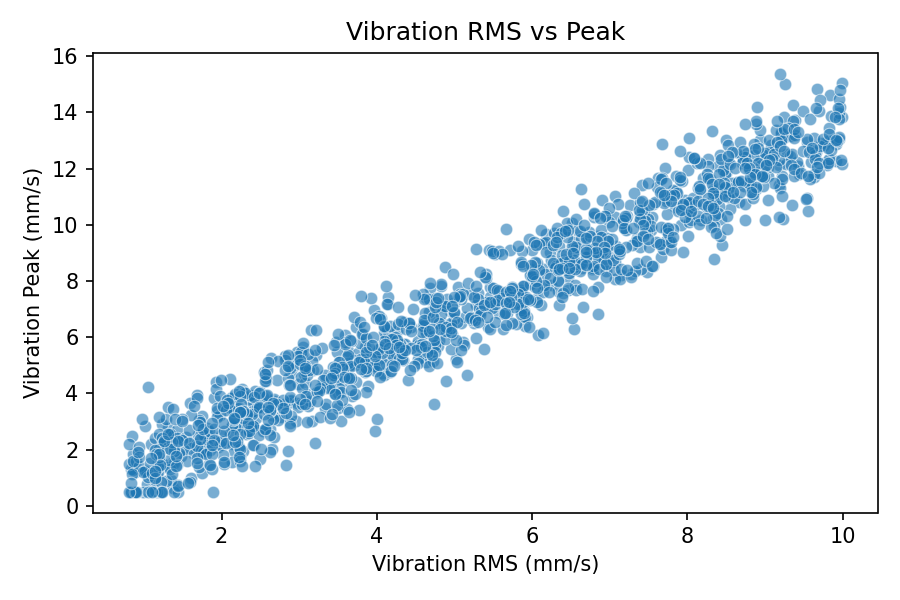
\includegraphics[width=0.75\textwidth]{img/vibration_scatter.png}
        \vspace{0.5em}

        The two vibration features are strongly related, which may introduce some redundancy.
    \end{frame}
    \section{Modeling}
    \begin{frame}
        \frametitle{Constant Predictor as a Baseline}
        \begin{itemize}
            \item The baseline always predicts the majority class, i.e., non-failure of the machine.
            \item High accuracy observed (0.866), but not representative because of class imbalance.
            \item Balanced accuracy of 0.5, indicating no ability to distinguish failures from non-failures.
            \item PR-AUC of 0.134, exactly the failure rate: the score of a model with no information.
            \item Conclusion: accuracy is out; PR-AUC is our primary metric.
        \end{itemize}
    \end{frame}
    \begin{frame}
        \frametitle{Evaluation Protocol}
        \begin{itemize}
            \item All comparisons use stratified 5-fold cross-validation on the training file, preserving the 13.4\% failure rate in every fold.
            \item Scaling lives inside a pipeline, fit on each fold's training part only: no data leakage.
            \item Hyperparameters are selected by cross-validation, never on the test set.
            \item The test file is opened exactly once, after the model and the threshold are frozen.
        \end{itemize}
    \end{frame}
    \begin{frame}
        \frametitle{Candidate Models}
        \begin{itemize}
            \item Logistic regression: plain, with balanced class weights, and with a tuned L2 penalty
            \item Linear discriminant analysis
            \item Gaussian Naive Bayes
            \item K-nearest neighbors, with $k$ tuned by cross-validation
        \end{itemize}
        \vspace{0.5em}
        All methods from the course material; each makes a different assumption about how features relate to failure.
    \end{frame}
    \begin{frame}
        \frametitle{K-Nearest Neighbors}
        \centering
        \includegraphics[width=0.7\textwidth]{img/knn_k_selection.png}
        \begin{itemize}
            \item Scaling is mandatory: distances would otherwise be dominated by large-magnitude features.
            \item Best $k = 101$: with only 13\% positives, small neighborhoods rarely contain a failure at all.
            \item CV PR-AUC 0.435. The ranking is fine, but at the default 0.5 cutoff kNN flags almost nothing.
        \end{itemize}
    \end{frame}
    \begin{frame}
        \frametitle{Logistic Regression}
        \begin{itemize}
            \item Penalty strength tuned by cross-validation ($C = 0.1$), the same selection problem as choosing $\lambda$ for Ridge.
            \item Balanced class weights compensate the imbalance during training.
            \item Best model in the comparison: CV PR-AUC $0.450 \pm 0.110$.
            \item Readable coefficients: prior failures, vibration, operating hours and machine age increase risk; operator experience decreases it.
        \end{itemize}
    \end{frame}
    \section{Policy and Evaluation}
    \begin{frame}
        \frametitle{Choice of Final Model}
        \begin{itemize}
            \item CV PR-AUC: logistic regression 0.450, LDA 0.438, kNN 0.435, Naive Bayes 0.430.
            \item Fold-to-fold standard deviation is 0.110: the top models overlap, so we cannot claim a statistically clear winner.
            \item With overlapping scores, we prefer the simpler, interpretable model: logistic regression, whose coefficients the reliability team can read.
            \item Naive Bayes has the highest ROC-AUC, but ROC-AUC is inflated by the large negative class; PR-AUC matches the task.
        \end{itemize}
    \end{frame}
    \begin{frame}
        \frametitle{A Preventive Policy}
        \centering
        \includegraphics[width=0.62\textwidth]{img/pr_operating_points.png}
        \begin{itemize}
            \item The threshold is the policy. We price six recall guarantees on out-of-fold predictions.
            \item From 0.70 to 0.80 recall: $\sim$7 extra inspections per additional failure caught; from 0.80 to 0.85: $\sim$15. Returns collapse.
            \item Chosen point: recall $\geq 0.80$ at $t = 0.43$. Any machine scoring above it is booked for the next planned downtime slot.
        \end{itemize}
    \end{frame}
    \begin{frame}
        \frametitle{Final Evaluation Results}
        \centering
        \includegraphics[width=0.45\textwidth]{img/test_confusion_matrix.png}
        \begin{itemize}
            \item Test set used once, threshold frozen: 33 of 37 failures caught (recall 0.89), 47\% of the fleet flagged, precision 0.20.
            \item PR-AUC 0.40 against a 10.6\% base rate: ranking almost four times better than random.
            \item Precision dip vs training folds is base-rate arithmetic (10.6\% vs 13.4\% failures), not model decay; ROC-AUC held at 0.82.
        \end{itemize}
    \end{frame}
    \begin{frame}
        \frametitle{Limitations and What the Model Misses}
        \begin{itemize}
            \item The missed failures look like healthy machines: near-healthy vibration and no failure over the last year. A limit of the sensors, not of the threshold.
            \item Snapshot data: the model cannot see trends such as vibration rising over weeks.
            \item Failure and maintenance costs are not in the data; the operating-point table lets FactoryPulse move the recall floor the day real costs exist, without retraining.
            \item The threshold assumes a stable failure rate: monitor the flag rate in production and re-pick from the table if it drifts.
        \end{itemize}
    \end{frame}
\end{document}
